\section{Method}\label{sec:Method}

\subsection{Yelp Data}
The goal of this project was to explore different classification algorithms to see how they perform on Yelp data and if they are able to classify if a business gets top rating or not. The methods explored were \textit{Logistic Regression} with \textit{Stochastic Gradient Descent}, \textit{Decision Trees}, \textit{Random Forest}, and \textit{AdaBoost}. The data is taken from the \href{https://www.yelp.com/dataset/challenge}{Yelp data challenge} which offers disparate datasets containing about 4.5 million reviews along with data about the business. A subset of \numprint{500 000} reviews were extracted and used in this analysis. The dataset was created by concatenating a subset of predictors from a business, a user and a review, with the \texttt{rating} variable of the review used as the response.

Considerable preprocessing was performed on the data, with the most important parts summarized listed below. A notebook is available in the GitHub repository to reproduce the preprocessing.
\begin{easylist}
& Preparing the data
&& The dataset contains information about the business which the customer can choose to give information about whilst rating. Some are deemed as categorical such as \texttt{restaurant\ take\ out}, \texttt{trendy} and \texttt{desserts}. These are encoded by  creating indicator columns for $NaN$, $True$ and $False$.
&& The quantitative predictors such as \texttt{review\ count} were shifted by their mean and scaled by their standard deviation.
&& Several predictors such as \texttt{postal code} and \texttt{city} were dropped as no good encodings were found. 
\end{easylist}

In  order to examine the distribution of \texttt{rating}, its values are plotted in~\ref{fig:binbar}.
At a glance it is clear that there are large class imbalances. Class imbalances have
been an active area of research the last decade, providing several methods to deal the problem.
To limit the complexity of this project, a simple solution was employed, namely rebinning the data so that the classes become more equal.
Whenever data is binned there is some arbitrariness introduced, unless one has a good
reason for it. It our case, it is reasonable to consider a 5 star rating as being "outstanding", a 1 star rating as "awful", and in-between ratings as different shades of "ok". Two reasonable binnings are therefore "outstanding" vs "non-outstanding" and
"outstanding" vs "ok" vs "awful.
The former was chosen and achieved by binning all ratings less than 5 into a single $< 5$ bin, as seen in the second panel of~\ref{fig:binbar}. The latter option was chosen against as the class imbalance problem remains unfixed. 
When splitting the data into training and test sets it was stratified so as to preserve the class ratios.

\begin{figure}[H]
    \begin{subfigure}
        \centering
        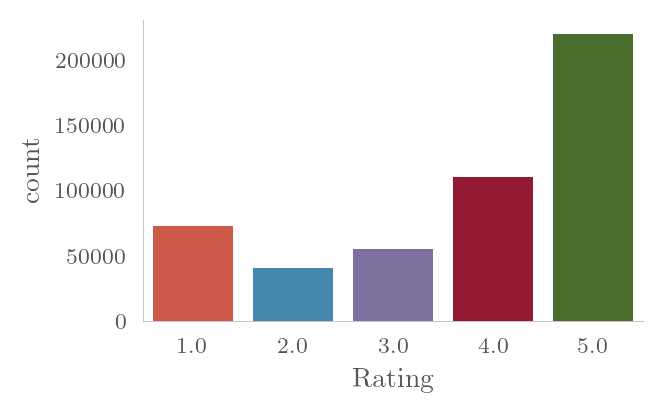
\includegraphics{Figures/rating.png}
        \caption{Distribution of review ratings.}
    \end{subfigure}
    \begin{subfigure}
        \centering
        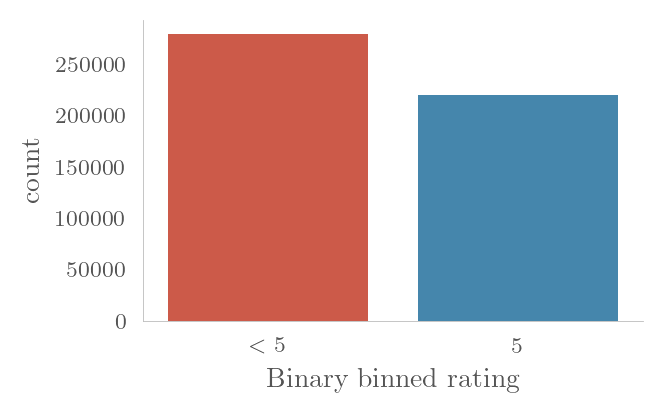
\includegraphics{Figures/rating_bin.png}
        \caption{Distribution of review ratings where $1, 2,3 ,4$ are binned
        into a single $<5$ bin}
    \end{subfigure}
    \begin{subfigure}
        \centering
        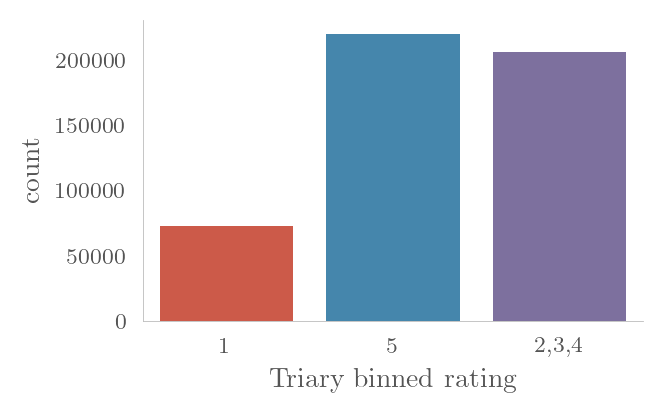
\includegraphics{Figures/rating_tri.png}
        \caption{Distribution of review ratings where $2,3 ,4$ are binned
        into a single bin. Ratings 1 and 5 are left undisturbed.}
    \end{subfigure}
    \label{fig:binbar}
\end{figure}

\subsubsection{Logistic Regression}
The implementation of logistic regression follows the theory in section \ref{subsec:LogRegTheory}. The only hyperparameter tuned was penalization type
($L_1$ vs $L_2$) and regularization strength. The error was decomposed using 
bootstraping.

\subsubsection{Random Forest and AdaBoost}\label{DecisionTrees}
These classification methods differ from the logistic regression because they 
are usually better and preferable when one has more than two classes. 
\begin{easylist}
& Scikit Learn implementation 
&& The Random Forest can also be applied as a function in the Scikit Learn Library RandomForestClassifier. A Random Forest is a meta estimator that fits a number of decision tree classifiers on various sub-samples of the dataset and uses averaging to improve the predictive accuracy and control over-fitting \cite{ScikitLRandom}. Again there are various parameters to choose from, some are the same as for Decision Trees, like the criterion parameter. Another is the $n \_estimators$ which decides how many trees there should be in the forest. In this project we first iterated over this parameter and evaluated it against the accuracy score to find the optimal number of trees for our dataset.
&& AdaBoost for classification, which in Scikit Learn has the name AdaBoostClassifier is also a meta estimator which firstly fits a classifier to the whole dataset but then also fits a copy of that classifier to the dataset and then aims to correct for incorrectly classified samples done by the first fit. So one of the parameters which is called $base\_estimator$ takes in the classifier that works as a base, say DecisionTreeClassifier, then the AdaBoost will literally boost the method trying to correctly classify the incorrect prediction of the Decision Tree method. 
& Evaluation
&& All methods above where evaluated by confusion matrices using the function $confusion\_matrix$. This to see how the different methods performed with the different classes mentioned above. 
\end{easylist}

All of the calculations can be reproduced by running the Jupyter notebooks.



